\begin{boiboiboite}
	\propeau
	\propair
	\isentropiques
	\isothermes
	\efficacitescarnot
\end{boiboiboite}


\subsubsection{Efficacité maximale d’un moteur}
\label{exo_efficacite_moteur_carnot}

	Quelle est l’efficacité maximale qu’une centrale à vapeur puisse atteindre en opérant dans l’atmosphère à température ambiante (\SI{15}{\degreeCelsius}), et dont le cycle a une température maximale de~\SI{800}{\degreeCelsius} ?

\subsubsection{Efficacité maximale d’un réfrigérateur}
\label{exo_efficacite_refrigerateur_carnot}

	Quelle est l’efficacité maximale théorique qu’un congélateur domestique pourrait atteindre en fonctionnant entre les températures de~\SI{-6}{\degreeCelsius} et~\SI{20}{\degreeCelsius} ?
	
	Pour quelle(s) raison(s) le \textsc{cop} atteint par les congélateurs usuels (environ \num{3}) sont-ils inférieurs ?
	
\subsubsection{Efficacité maximale d’une thermopompe}
\label{exo_efficacite_thermopompe_carnot}

	Une personne souhaite installer une pompe à chaleur pour chauffer son domicile avec une puissance de~\SI{10}{\kilo\watt}.

	\begin{enumerate}
	
		\item Expliquez brièvement pourquoi la performance d’une pompe à chaleur s’exprime selon :
			\begin{equation}
				\eta_\text{thermopompe} = \left| \frac{\dot Q_\out}{\dot W_\net} \right|
			\end{equation}

		\item Estimez la consommation minimale théorique de la pompe un soir de grand froid ($T_\text{ext.} = \SI{-12}{\degreeCelsius}$; $T_\text{int.} = \SI{20}{\degreeCelsius}$).
		
		\item Quelle sera la consommation minimale de la pompe à chaleur lorsque les températures interne et externe seront de~\SI{17}{\degreeCelsius}  et~\SI{16}{\degreeCelsius} respectivement ? 
		
		\item Quelle sera la consommation minimale théorique de la pompe dans le cas où les températures interne et externe sont identiques ?  Que se passe-t-il en théorie si la température externe est plus grande qu’à l’intérieur ?

	\end{enumerate}


\subsubsection{Cycle de Carnot}
\label{exo_cours_carnot}

	Comme ce cycle joue un rôle central en thermodynamique, il est utile de savoir le décrire précisément :
	
	\begin{enumerate}
	
		\item Décrivez brièvement les quatre phases d’un cycle moteur de Carnot, en décrivant le sens des transferts de chaleur.
	
		\item Pourquoi les transferts de chaleur sont-ils isothermes ?
		
		\item Est-il préférable d’utiliser un gaz parfait ou un mélange liquide-vapeur pour effectuer ce cycle ?
		
		\item Quels problèmes pratiques le cycle de Carnot pose-t-il ? 

	\end{enumerate}


\subsubsection{Moteur de Carnot à vapeur}
\label{exo_moteur_carnot_vapeur}
% Cet exo est lié à l’exercice 8.5 (\ref{exo_diagrammes_ts})

	On tente de mettre en place une centrale à vapeur basée sur le cycle de Carnot pour fabriquer de l’électricité (\cref{fig_exo_carnot_circuit_vapeur}). La chaudière fonctionne à température maximale de~\SI{275}{\degreeCelsius} et admet de l’eau à l’état de liquide saturé. Lorsque l’eau sort de la chaudière et rentre dans la turbine, elle est à l’état de vapeur saturée.

	\begin{figure}[hc]%FIXME handmade, fuck, why can I not have the figure display here?!
		\begin{center}
			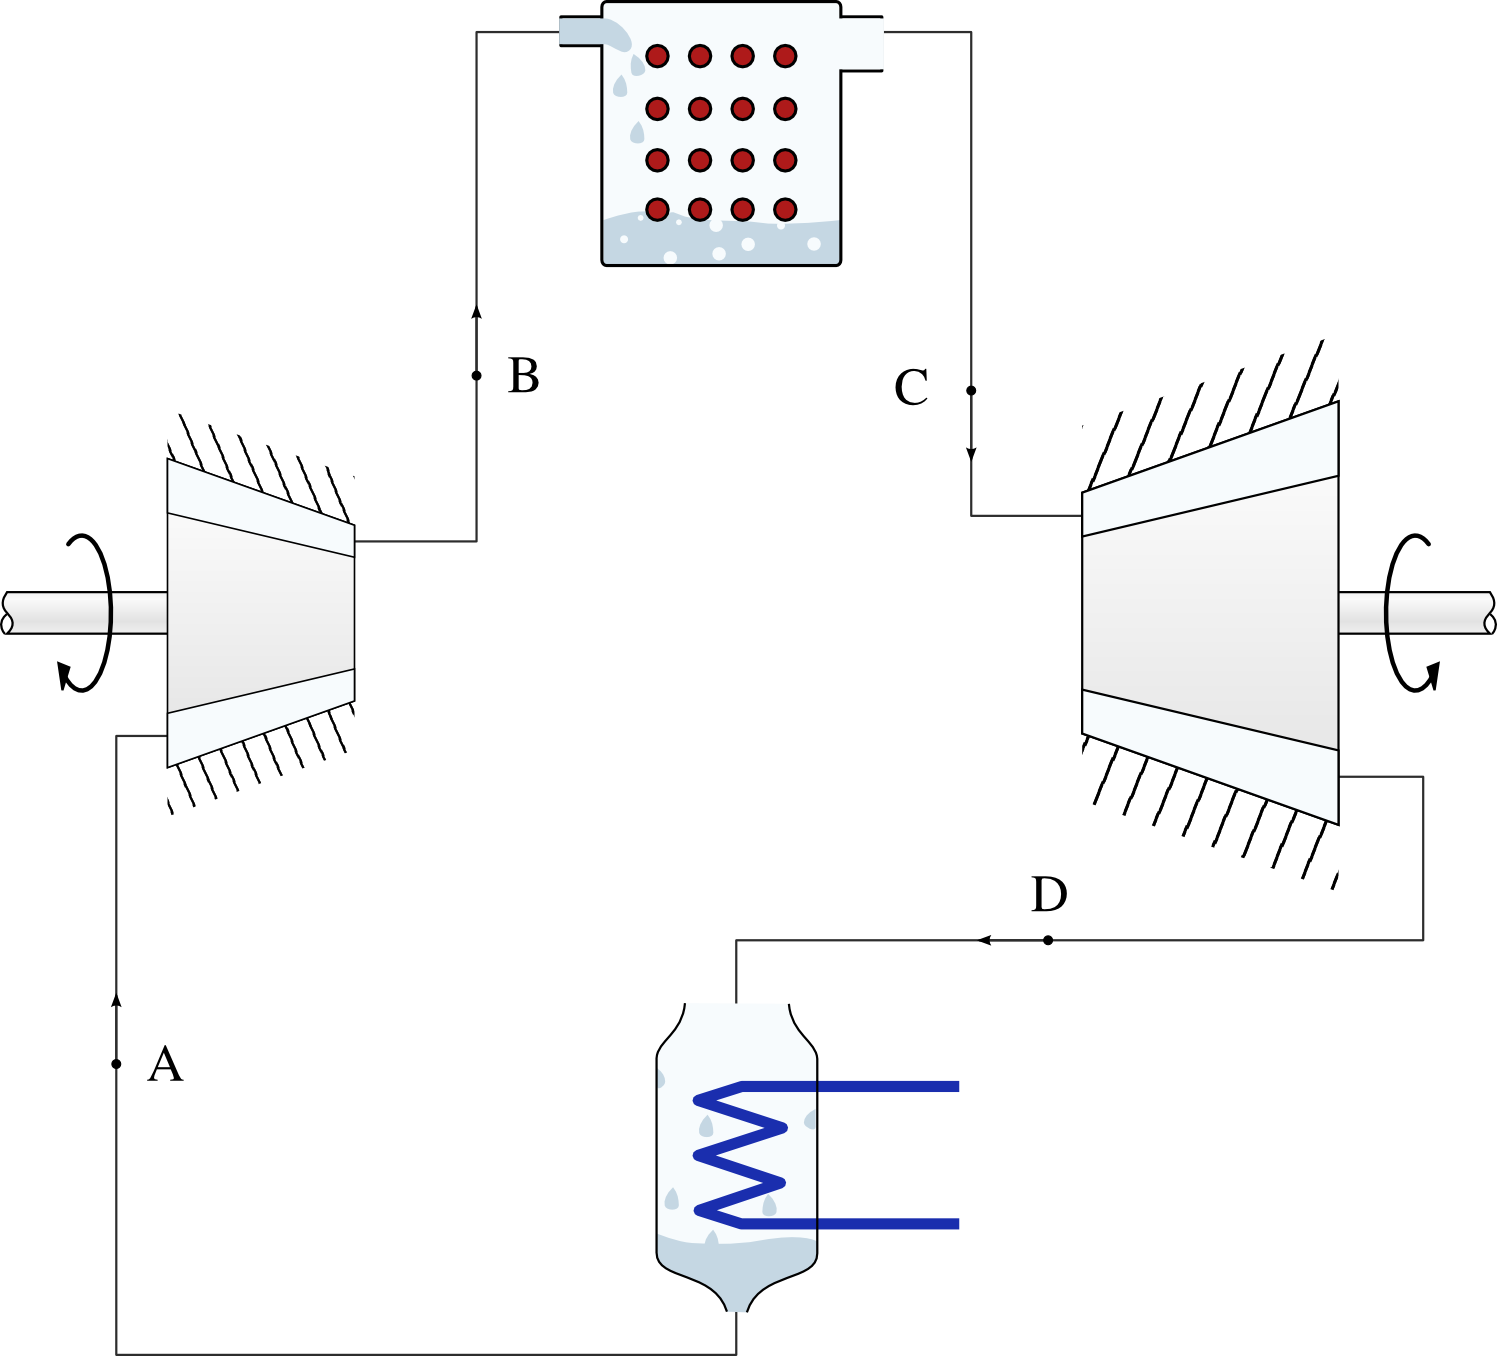
\includegraphics[width=7cm]{images/circuit_carnot_vapeur.png}
		\end{center}
		\supercaption{Représentation schématique d’une centrale à vapeur fonctionnant avec le cycle de Carnot.}{schéma \ccbysa \olivier}
		\label{fig_exo_carnot_circuit_vapeur}
	\end{figure}
	
	\begin{enumerate}
	
		\item Tracez le cycle suivi par l’eau sur un diagramme pression-volume, de façon qualitative (c’est-à-dire sans représenter les valeurs numériques) et en y indiquant la courbe de saturation.
		
		\item À quelle pression faudrait-il refroidir l’eau pour obtenir un rendement de~\SI{40}{\percent} ?
		
		\item Quelle serait la puissance fournie par l’installation si son débit massique était de~\SI{9}{\kilogram\per\second} ?
		
		\item À quoi ressembleraient le cycle et la machine si l’on continuait à chauffer la vapeur à température constante de~\SI{275}{\degreeCelsius} à la sortie de la chaudière ? Comment varierait alors l’efficacité du moteur ?
		
	\end{enumerate}


\subsubsection{Réversibilité des machines}
\label{exo_thermopompe_plusplus}

	Montrez brièvement que l’on ne peut pas concevoir de pompe à chaleur de rendement supérieur à celui atteint par une machine réversible, par exemple de la même façon que nous l’avons fait avec un moteur en \cref{fig_plus_que_machine_de_carnot}.


\subsubsection{Moteur à turbine idéal}
\label{exo_moteur_turbine_ideal}
\wherefrom{[DS n°2 2012, 11pts]}
% Cet exo est lié à l’exercice 8.5 (\ref{exo_diagrammes_ts})

	Un groupe d’ingénieurs dans un bureau d’études travaille sur la conception d’un moteur à air, fonctionnant en régime continu à l’aide de turbines et de compresseurs.

	Les ingénieurs utilisent le cycle de Carnot pour point de départ. Ils prévoient de pouvoir effectuer l’apport de chaleur à température de~\SI{600}{\degreeCelsius} et le rejet de chaleur à température de~\SI{20}{\degreeCelsius}. La pression est de~\SI{1}{\bar} à l’entrée du compresseur adiabatique et de~\SI{30}{\bar} à l’entrée de la turbine adiabatique. Ces caractéristiques confèrent au moteur une puissance mécanique spécifique de~\SI{70}{\kilo\joule\per\kilogram}.

	\begin{enumerate}
		\item Représentez l’agencement général de ce moteur hypothétique, en y représentant le circuit suivi par l’air, et tous les transferts de chaleur et de travail.
		\item À partir de la définition du rendement d’un moteur, montrez que l’efficacité d’un moteur réversible est quantifiable selon l’équation
			\begin{equation}
				\eta_{\text{moteur Carnot}} = 1 - \frac{T_B}{T_H} \tag{\ref{eq_efficacité_moteur_carnot_température}}
			\end{equation}
		\item Quelle puissance sous forme de chaleur faudra-il fournir au moteur ?
		\item Quelle sera alors la puissance rejetée sous forme de chaleur ?
	\end{enumerate}

	Bien sûr, le cycle de Carnot est impraticable dans une application industrielle et le groupe d’ingénieurs adopte immédiatement une modification, car pour pouvoir effectuer l’apport de chaleur par combustion interne, il est nécessaire de vidanger ensuite l’air du moteur. Ainsi, dans le moteur modifié, la détente dans la turbine adiabatique est interrompue lorsque la pression atteint \SI{1}{\bar}, et l’air «~usagé~» est alors rejeté dans l’atmosphère. Le reste du moteur n’est pas affecté.
	
	\begin{enumerate}
		\shift{4}
		\item Représentez le cycle du moteur sur un diagramme pression-volume, de façon qualitative, en le comparant à celui du cycle de Carnot.
		\item Quelle est la température de l’air lorsqu’il est rejeté du moteur ?
		\item Quelle est ainsi la réduction de la puissance de la turbine adiabatique par rapport au moteur idéal ?
		\item Quelle puissance mécanique est économisée par la suppression du compresseur qui effectuait le rejet de chaleur ?
		\item Quelle est désormais l’efficacité du moteur ?
	\end{enumerate}


\subsubsection{Cycle idéal et réel d’un réfrigérateur}
\label{exo_cours_refrigerateur_carnot}
\wherefrom{[DS n°2 2011, 4pts]}

	Nous nous proposons d’étudier le fonctionnement d’un réfrigérateur en partant d’un cycle théorique permettant un rendement maximal.
	
	Le réfrigérateur fonctionne strictement sur un cycle de Carnot, en régime permanent, avec un mélange liquide-vapeur.
	
	\begin{enumerate}
		\item Représentez le cycle de réfrigération sur un diagramme pression-volume, en indiquant le sens des transferts de chaleur et de travail.
	\end{enumerate}
	
	Bien sûr, en pratique, la compression et la détente adiabatiques ne peuvent pas être effectuées de façon réversible.
	
	\begin{enumerate}
		\shift{1}
		\item Représentez le cycle irréversible sur le diagramme pression-volume.
		\item De quelle façon variera chacun des transferts de chaleur et de travail par rapport au cas théorique ?
		\item Montrez brièvement que ces variations conduisent à une baisse du rendement (le \textsc{cop}) du réfrigérateur.
	\end{enumerate}


\subsubsection{Réfrigération par étages}
\label{exo_refrigeration_etages}
\wherefrom{[DS n°2 2012, 7pts]}

	Une usine chimique utilise un système de réfrigération pour contrôler la température de produits dangereux. Nous cherchons à étudier le système de réfrigération le moins inefficace pour l’équiper, ici basé sur le cycle de Carnot avec un gaz parfait.
	
	La température minimale de réfrigération est de~\SI{-50}{\degreeCelsius} et la chaleur est rejetée à~\SI{40}{\degreeCelsius}.
			
	En étudiant les propriétés du cyle de Carnot, un/e ingénieur/e débutant/e constate que le rendement du réfrigérateur augmente si la température de rejet de chaleur est abaissée.
	
	Il/elle propose de configurer le réfrigérateur de telle sorte à ce qu’il rejette de la chaleur à~\SI{10}{\degreeCelsius} seulement. Cette chaleur à~\SI{10}{\degreeCelsius} serait à son tour captée par une pompe à chaleur qui la mènerait enfin à~\SI{40}{\degreeCelsius}. 
	
		\begin{enumerate}
			\item Montrez que le si le réfrigérateur fonctionne sur un cycle réversible, la modification proposée ne pourra qu’augmenter (ou au mieux, garder identique) la consommation totale du système de réfrigération.
			\item Représentez le cycle du réfrigérateur et de la pompe à chaleur telle que le propose l’ingénieur/e, sur un même diagramme pression-volume, de façon qualitative.
			\item Représentez, sur un diagramme pression-volume, les cycles qui seraient suivis dans les deux machines si leurs phases de détentes étaient adiabatiques (sans transfert de chaleur) mais non-réversibles.
		\end{enumerate}


\subsubsection{Moteur essence basé sur un cycle de Carnot}
\label{exo_carnot_quatre_cylindres}

	On souhaite quantifier la consommation d’essence minimale que pourrait engendrer un moteur automobile à pistons-cylindres générant \SI{100}{\kilo\watt} de puissance (environ \SI{130}{ch}), étant données quelques contraintes pratiques imposées par le faible volume disponible et les limites de poids :
		
	\begin{itemize}
		\item Le taux de compression (c’est-à-dire le rapport $\frac{v_\text{max.}}{v_\text{min.}}$) est de~\num{12} lors des phases adiabatiques (afin de limiter les contraintes mécaniques) ;
		\item La température maximale est de~\SI{1300}{\kelvin} (imposée par la résistance des matériaux) ;
		\item Le moteur a quatre cylindres effectuant chacun \num{400} cycles par minute.
	\end{itemize}
	
	Le moteur est alimenté par de l’essence dont la chaleur spécifique de combustion est de~\SI{40}{\mega\joule\per\kilogram}.
	
	Si l’on considère le meilleur moteur que l’on puisse concevoir :
	
	\begin{enumerate}
		\item À quelle température la chaleur serait-elle rejetée ?
		\item Quel serait le rendement du moteur ?
		\item Quelle serait la quantité de chaleur à fournir pour chaque combustion, et la masse de carburant correspondante ?
		\item Quelle serait la consommation horaire d’essence ?
	\end{enumerate}

\exercisesolutionpage
\titreresultats

	\begin{description}
		\item [\ref{exo_efficacite_moteur_carnot}] 
					\tab $\eta_\text{max.} = \SI{73,1}{\percent}$ (\ref{eq_efficacité_moteur_carnot_température}, cf. exemple~\ref{ex_efficacite_moteur_carnot}).
		\item [\ref{exo_efficacite_refrigerateur_carnot}] 
					\tab 1) $\textsc{cop}_\text{max.} = \num{10,3}$ (\ref{eq_efficacité_réfrigérateur_carnot_température}, cf. exemple~\ref{ex_efficacite_refrigerateur_carnot}) ;
					\tab 2) Compressions et détentes non réversibles (ainsi $w_{4\to 3} + w_{2\to 1} > 0$), en particulier si une soupape est utilisée (\S\ref{ch_principe_fonctionnement_réfrigérateur}) ; échanges de chaleur non-isothermes.
		\item [\ref{exo_efficacite_thermopompe_carnot}]
					\tab 1) cf. \S\ref{ch_rendement_thermopompe}	;
					\tab 2) $\dot W_\net = \frac{\dot Q_\out}{\eta_\text{max.}} = \SI{+1,09}{\kilo\watt}$ ;
					\tab 3) $\dot W_\net = \SI{+34,5}{\watt}$ (!) 
					\tab 4) $\dot W_\net = \SI{0}{\watt}$ ; et lorsque $T_\text{ext.} > T_\text{int.}$, $\dot W_\net$ devient négatif : la thermopompe fonctionne comme un moteur…
		\item [\ref{exo_cours_carnot}]
					\tab 1) cf. \S\ref{ch_descritpion_cycle_carnot}, et en particulier les figures~\ref{fig_carnot_quatre_etapes} et~\ref{fig_carnot_quatre_etapes_so} ;
					\tab 2) cf. \S\ref{ch_elaboration_cycle_carnot} ;
					\tab 3) Cela n’a aucune importance !
					\tab 4) Son encombrement, son rapport des puissances sont très grands, et sa puissance est infiniment faible…
		\item [\ref{exo_moteur_carnot_vapeur}] 
					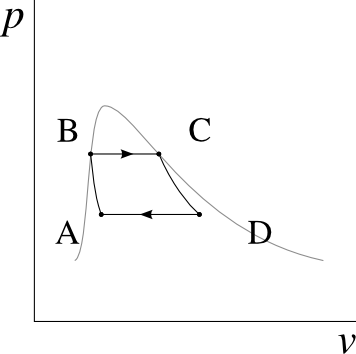
\includegraphics[width=\solutiondiagramwidth]{images/exo_sol_pv_carnot_lv_1.png}
					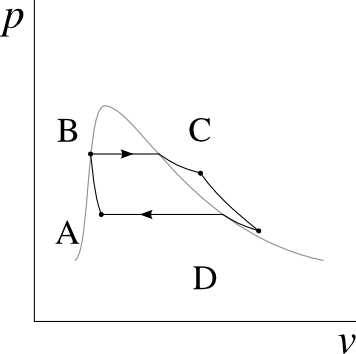
\includegraphics[width=\solutiondiagramwidth]{images/exo_sol_pv_carnot_lv_2.png}
					Nous voyons que lorsqu’il est effectué sous la courbe de saturation, le cycle de Carnot est déjà moins complexe à réaliser en pratique, puisque les échanges de chaleur se font à pression constante (et ne nécessitent ainsi pas de pièce mobile)  ;
					\tab 2) $T_B = (1 - \eta) T_H = \SI{55,74}{\degreeCelsius}$ ; ainsi par interpolation entre \num{55} et \SI{60}{\degreeCelsius} on obtient $p_\text{sat. \SI{55,74}{\degreeCelsius}} = \SI{0,1285}{\bar}$. Le condenseur est donc dépressurisé  ;
					\tab 3) $q_\inn = h_{LV\SI{275}{\degreeCelsius}} = \SI{+1574,3}{\kilo\joule\per\kilogram}$ : on obtient $\dot W_\net = -\dot m \eta q_\inn = \SI{-566,7}{\kilo\watt}$  ;
					\tab 4) La puissance spécifique et la complexité de la machine augmenteront, mais l’efficacité sera inchangée !
		\item [\ref{exo_thermopompe_plusplus}]
					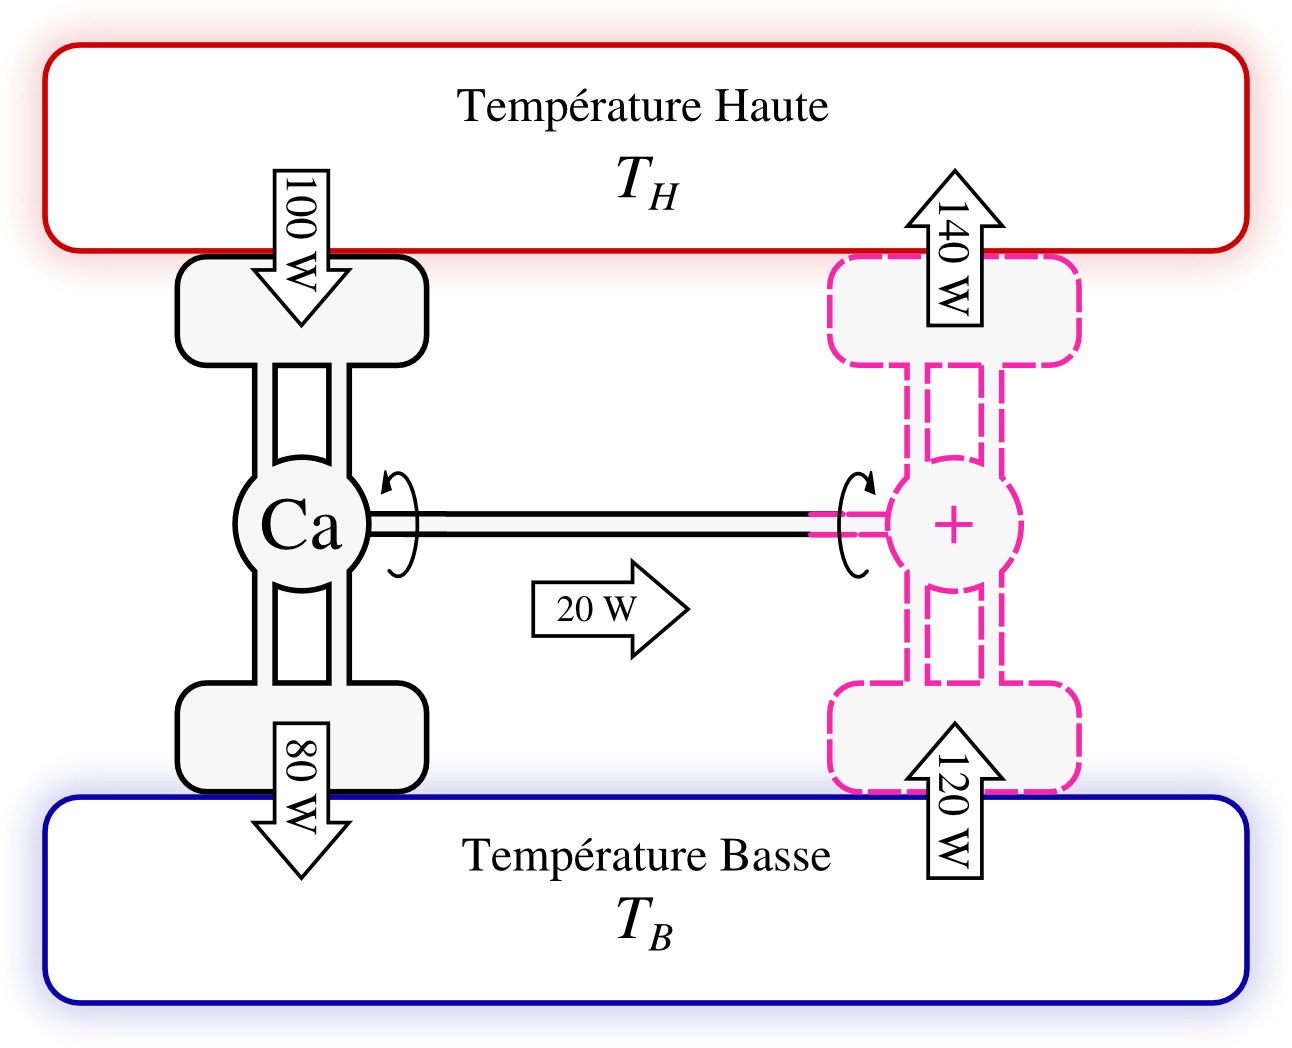
\includegraphics[width=5cm]{images/carnot_thermopompe_plusplus.png}
					\tab\tab Une telle pompe à chaleur pourrait être alimentée par un moteur de Carnot ; l’ensemble formerait une machine capable de porter de la chaleur depuis $T_B$ jusqu’à $T_H$ sans apport de travail extérieur (avec les valeurs arbitraires motrées ici, $\dot Q_{\out \text ensemble} = \SI{-40}{\watt}$).
		\item [\ref{exo_moteur_turbine_ideal}]
					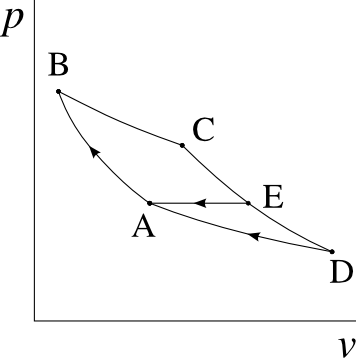
\includegraphics[width=\solutiondiagramwidth]{images/exo_sol_pv_carnot_turbine.png}
					\tab 1) C’est l’agencement représenté en \cref{fig_carnot_quatre_etapes_so} ;
					\tab 2) En partant de l’\cref{def_rendement_moteur}  : $\eta_\text{moteur} 
						\equiv \left| \frac{\dot W_\net}{\dot Q_\inn} \right|
						= - \frac{\dot W_\net}{\dot Q_\inn}
						= - \frac{-\dot Q_\inn - \dot Q_\out}{\dot Q_\inn}
						= 1 + \frac{\dot Q_\out}{\dot Q_\inn}
						= 1 - \left|\frac{\dot Q_\out}{\dot Q_\inn}\right| 
						= 1 - \left|\frac{\dot Q_{TH}}{\dot Q_{TB}}\right|$ ; Avec la définition \ref{def_échelle_température_kelvin} on arrive à l’\cref{eq_efficacité_moteur_carnot_température} demandée ;
					\tab 3) ${q}_\inn = -\frac{w_\net}{\eta_\text{moteur}} = \SI{+105,4}{\kilo\joule\per\kilogram}$ ;
					\tab 4) ${q}_\out = -w_\net - q_\inn = \SI{-35,4}{\kilo\joule\per\kilogram}$ ;
					\tab 6) Le compresseur isotherme est supprimé, la turbine adiabatique est tronquée. $T_E = T_C \left(\frac{p_E}{p_C}\right)^\frac{\gamma - 1}{\gamma} = \SI{330,4}{\kelvin} = \SI{57,3}{\degreeCelsius}$ (\ref{eq_isentropique_horrible2}) ;
					\tab 7) $w_\text{perdue} = w_\text{turbine isentropique 1} - w_\text{turbine isentropique 2} = \SI{-37,54}{\kilo\joule\per\kilogram}$ ;
					\tab 8) $w_\text{économisée} = w_\text{compresseur isentropique} = \SI{+35,4}{\kilo\joule\per\kilogram}$ ;
					\tab 9) $\eta_\text{moteur 2} = \SI{64,4}{\percent}$, soit \SI{-2}{points}, fort honorable au vu de la simplification considérable de la machine !
		\item [\ref{exo_cours_refrigerateur_carnot}]
					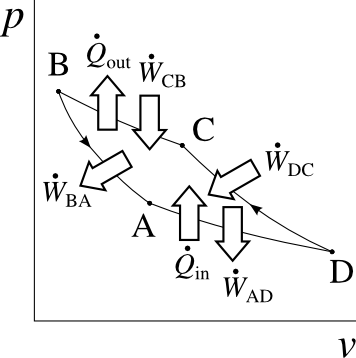
\includegraphics[width=\solutiondiagramwidth]{images/exo_sol_pv_carnot_refrigerateur_transferts.png}
					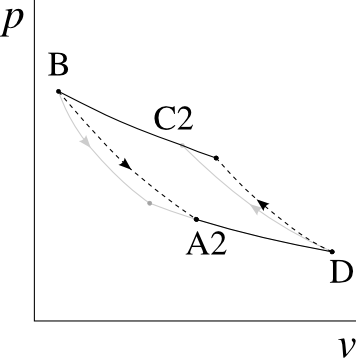
\includegraphics[width=\solutiondiagramwidth]{images/exo_sol_pv_carnot_refrigerateur_irreversibilites.png}
					\tab 3) $w_{1\to 4}$ diminue, $w_{4\to 3}$ et $w_{3\to 2}$ augmentent, $w_{2\to 1}$ diminue ; $q_{3\to 2}$ augmente et $q_{1\to 4}$ diminue  ;
					\tab 4) Comme $w_\net$ augmente et que $q_\inn = q_{1\to 4}$ diminue, le $\textsc{cop} = \frac{q_\inn}{w_\net}$ diminue nécessairement.
		\item [\ref{exo_refrigeration_etages}]
					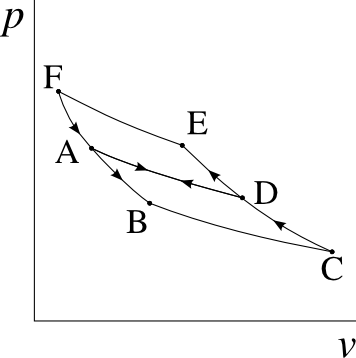
\includegraphics[height=\solutiondiagramwidth]{images/exo_sol_pv_refrigeration_etages_1.png}
					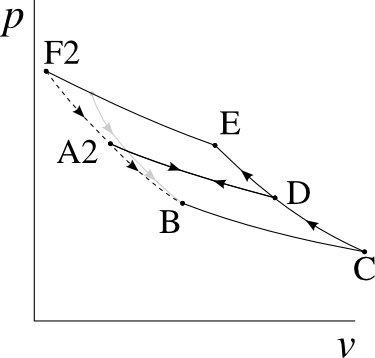
\includegraphics[height=\solutiondiagramwidth]{images/exo_sol_pv_refrigeration_etages_2.png}
					\tab 1) Gageons que l’étudiant/e aura fait mieux que l’ingénieur/e débutant/e de l’exercice : avec deux systèmes réversibles en série pompant une quantité $q_\inn$ de chaleur à température $T_1 = \SI{-50}{\degreeCelsius}$, avec température d’échange $T_2 = \SI{10}{\degreeCelsius}$ et température haute finale $T_3 = \SI{40}{\degreeCelsius}$, le travail nécessaire est $w_\text{total} 
						= w_{\net1} + w_{\net2}
						= \eta_1 q_\inn + \eta_2 (q_\inn + w_{\net1})
						= \left(\frac{T_2}{T_1} - 1\right) q_\inn \ + \ \left(\frac{T_3}{T_2} - 1\right) (q_\inn + w_{\net1})
						= \left(\frac{T_2}{T_1} - 1\right) q_\inn \ + \ \left(\frac{T_3}{T_2} - 1\right) (q_\inn + \left(\frac{T_2}{T_1} - 1\right) q_\inn)
						= \left(\frac{T_2}{T_1} - 1\right) q_\inn \ + \ \left(\frac{T_3}{T_2} - 1\right) (\frac{T_2}{T_1} q_\inn)$ ; 
						ainsi $\eta_\text{ensemble} \equiv \frac{q_\inn}{w_\text{total}}
						= \frac{1}{\frac{T_2}{T_1} - 1 + \frac{T_3 T_2}{T_2 T_1} - \frac{T_2}{T_1}}
						= \frac{1}{\frac{T_3}{T_1} - 1}$, ce qui est l’efficacité d’une seule machine réversible fonctionant entre $T_1$ et $T_3$. L’échelonnage de deux machines en série n’apporte donc aucun avantage théorique.
		\item [\ref{exo_carnot_quatre_cylindres}]
					\tab 1) $T_\text{rejet} = T_1 = \SI{208}{\degreeCelsius}$ (\ref{eq_isentropique_horrible2}) ;
					\tab 2) $\eta_\text{moteur} = \SI{63}{\percent}$ ;
					\tab 3) $\dot Q_\inn = \SI{158,8}{\kilo\watt}$ donc $Q_\text{combustion 1 cylindre} = \SI{5,955}{\kilo\joule}$ à chaque combustion. On obtient, pour un cylindre, ${m}_\text{carburant combustion} = \frac{Q_\text{combustion 1 cylindre}}{q_\text{carburant}} = \SI{0,149}{\gram}$ ;
					\tab 4) $\dot{m}_\text{carburant} = \SI{14,3}{\kilogram\per\hour}$.
	\end{description}
